% ---
% school: "college"
% level: "8eme"
% section: null
% chapter: "التناظر المركزي"
% source: "Axiomaths"
% title: "مثلث متقايس الضلعين ومناظره"
% country: "Tunisie"
% year: 2026
% professor: "Axiomaths"
% difficulty: "Moyen"
% points: null
% tags: ["symetrie-centrale", "triangle-isocele", "losange", "angles"]
% ---
% Exercice 11/15 de la série 8ème « التناظر المركزي » (statement + \axsol + solution). Compiler avec XeLaTeX + axiomath.sty (+ axiomaths-logo.png).
\documentclass[12pt,a4paper]{article}
\usepackage[level=8b,color=15803D]{axiomath}
\usetikzlibrary{arrows.meta}
\newcommand{\cm}{\,\mathrm{cm}}
\axsetup{title={التناظر المركزي}, corrige}

\begin{document}

\begin{corr}[title={مثلث متقايس الضلعين ومناظره}, stars=3, source={Axiomaths}]
$ABC$ مثلث متقايس الضلعين رأسه $A$ حيث $\widehat{BAC}=40^\circ$. $I$ منتصف $[BC]$ و $D$ مناظرة $A$ بالنسبة إلى $I$.
\begin{enumerate}
  \item ابنِ الشكل.
  \item بين أن $ABDC$ متوازي أضلاع.
  \item بين أن $ABDC$ معين.
  \item احسب قيس كل من $\widehat{ABC}$ و $\widehat{BDC}$ و $\widehat{DBC}$.
  \item استنتج قيس الزاوية $\widehat{ABD}$.
\end{enumerate}
\axsol
\begin{enumerate}[itemsep=14pt]
  \item نبني $ABC$ ثم نعيّن $D$ بحيث $I$ منتصف $[AD]$.
  \begin{center}
  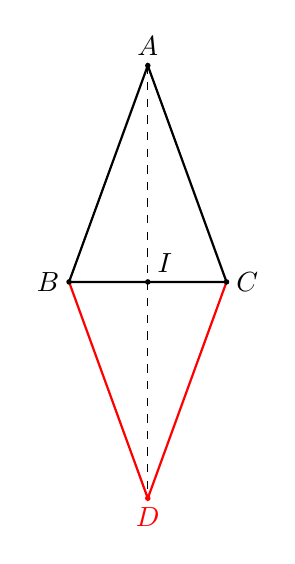
\begin{tikzpicture}[scale=0.5]
    \draw[thick] (-2,0)--(0,5.495)--(2,0)--cycle;
    \draw[thick,red] (-2,0)--(0,-5.495)--(2,0);
    \draw[dashed] (0,5.495)--(0,-5.495);
    \fill (0,5.495) circle (2pt) node[above] {$A$};
    \fill (-2,0) circle (2pt) node[left] {$B$};
    \fill (2,0) circle (2pt) node[right] {$C$};
    \fill (0,0) circle (2pt) node[above right] {$I$};
    \fill[red] (0,-5.495) circle (2pt) node[below] {$D$};
  \end{tikzpicture}
  \end{center}
  \item قطرا $ABDC$ هما $[AD]$ و $[BC]$ ، ولهما نفس المنتصف $I$ (لأن $D=S_I(A)$ و $I$ منتصف $[BC]$). إذن $ABDC$ متوازي أضلاع.
  \item $S_I$ يحوّل $A$ إلى $D$ و $B$ إلى $C$ و $C$ إلى $B$ ، فيحوّل $[AB]$ إلى $[DC]$ و $[AC]$ إلى $[DB]$. إذن $DC=AB$ و $DB=AC$. وبما أن $AB=AC$ :
  \[AB=BD=DC=CA\]
  لمتوازي الأضلاع $ABDC$ أضلاع أربعة متقايسة : إنه \ib{معين}.
  \item في المثلث المتقايس الضلعين $ABC$ زاويتا القاعدة متقايستان :
  \[\widehat{ABC}=\dfrac{180^\circ-40^\circ}{2}=70^\circ\]
  التناظر $S_I$ يحفظ قيس الزوايا ويحوّل $B$ إلى $C$ و $A$ إلى $D$ و $C$ إلى $B$ :
  \begin{itemize}
    \item الزاوية $\widehat{BAC}$ تُحوَّل إلى $\widehat{CDB}$ ، إذن $\widehat{BDC}=40^\circ$.
    \item الزاوية $\widehat{ACB}$ تُحوَّل إلى $\widehat{DBC}$ ، إذن $\widehat{DBC}=70^\circ$.
  \end{itemize}
  \item الشعاع $[BC)$ يقع بين $[BA)$ و $[BD)$ ، إذن :
  \[\widehat{ABD}=\widehat{ABC}+\widehat{CBD}=70^\circ+70^\circ=140^\circ\]
  \ib{زوايا المعين $ABDC$} هي : $40^\circ$ و $140^\circ$ و $40^\circ$ و $140^\circ$.
\end{enumerate}
\end{corr}

\end{document}
